\documentclass[12pt]{article}
\usepackage[margin=1in]{geometry}
\usepackage{amsmath,amssymb,amsthm,booktabs,graphicx,natbib,microtype}
\newtheorem{theorem}{Theorem}
\newtheorem{corollary}[theorem]{Corollary}
\newtheorem{proposition}[theorem]{Proposition}
\newtheorem{remark}[theorem]{Remark}
\title{Dyadic Packet-Transport Gauges\\\large Natural Exact-Gram Lifts and the Geometry--Tail Coherence Barrier}
\author{Prime Dynamics Theory Program}
\date{July 2026}

\begin{document}
\maketitle

\begin{abstract}
RH-132 constructed the polar partial isometry between two given supports,
but did not derive those supports from the model.  Here the gauge is made
dynamical and interscale.  The frozen Gaussian models already carry a
canonical dyadic isometry $J$ from a coarse source-coordinate space to the
next fine one.  At each selected phase, the memory recursion and adaptive
packet update produce an intrinsic four-frame $U_\sigma$.  We align
$JU_\sigma$ to $U_{\sigma/2}$ by the overlap polar factor $O_\sigma$ and
lift it to the exact-Gram gauge
\[
 S_\sigma=G_\sigma^{-1/2}O_\sigma^*G_{\sigma/2}^{1/2},
 \qquad
 S_\sigma^*G_\sigma S_\sigma=G_{\sigma/2}.
\]
This is the first cross-scale gauge in the route determined by the model's
grid and packet dynamics rather than by tail minimization.

The construction has a sharp limitation.  Its tail factor is always at
least the exact-Gram minimax factor, and no bound in terms of principal
angles alone is possible: even identical packet frames can have natural to
optimal tail-factor ratio $1/\varepsilon$.  A sufficient replacement is a
relative-tail coherence estimate in the natural frame.

The floor-free five-scale audit contains 96 phase-matched pairs.  Thirty are
zero-tail vacuous pairs, 24 are rank-birth pairs with infinite factor, and 42
have nonzero source and target tails.  The natural gauge preserves 35 of the
37 positive transport-eligible pairs, hence 65 positive transfers overall
versus 67 for the post-hoc optimum.  On the 42 eligible pairs, however, its
factor loss has median $10^{1.867}\approx73.7$ and maximum
$10^{9.987}$.  The minimum principal cosine and logarithmic loss have sample
correlation only $-0.174$.  Thus the natural gauge is surprisingly viable
for positivity, but a new tail-coherence law---not merely packet-angle
coherence---is required for uniform theory.
\end{abstract}

\section{From an abstract support map to a model-defined gauge}
The source-coordinate widths in the frozen family double when
$\sigma$ is halved.  The model construction uses the isometric coarse
embedding
\[
 J_m e_j=2^{-1/2}(e_{2j}+e_{2j+1}),
 \qquad J_m^*J_m=I.
\]
This is not an invented comparison map: it is the same dyadic embedding used
to form the coarse and detail blocks of the Gaussian operator.  It therefore
supplies a canonical identification between adjacent source-coordinate
spaces.

At a fixed scale and time, let $V$ be the recursively refreshed packet and
let $F$ be the leading four right singular frame of the projected recent
cross action.  The ambient input frame
\[
 U=VF
\]
is orthonormal and depends only on the source seed, memory recursion, packet
update, and chosen four-direction rule.  For adjacent scales define
\[
 C=U_{\sigma/2}^*J U_\sigma=L\Sigma R^*.
\]
The source-to-target polar alignment is $O_{st}=LR^*$ and the reduced
target-to-source alignment is $O=O_{st}^*$, the standard polar/Procrustes
choice for two frames \citep{GolubVanLoan2013}.

\section{Exact-Gram metric lift}
The geometric frames and the action metrics contain different information.
The polar factor aligns packet directions, while the positive Gramians
$G_\sigma=A_\sigma^*A_\sigma$ measure their action size.  They combine by a
canonical metric lift.

\begin{theorem}[Natural exact-Gram lift]\label{thm:lift}
Let $G,G'\succ0$ and let $O$ be any orthogonal target-to-source alignment.
Then
\[
 S=G^{-1/2}O(G')^{1/2}
\]
satisfies $S^*GS=G'$.  It is the unique exact-Gram lift whose normalized
orthogonal factor is $O$.  Moreover
\[
 |\det S|=\sqrt{\det G'/\det G}.
\]
\end{theorem}
\begin{proof}
Direct multiplication gives
$S^*GS=(G')^{1/2}O^*O(G')^{1/2}=G'$.  Conversely, normalizing any exact-Gram
gauge by $G^{1/2}S(G')^{-1/2}$ gives an orthogonal matrix, so fixing it to
$O$ fixes $S$.  Taking determinants proves the last identity.
\end{proof}

Thus the dyadic packet geometry determines one distinguished member of the
exact-Gram gauge family.  Unlike the RH-121 gauge, it does not inspect the
tail eigenspaces before choosing its orthogonal factor.  The positive-matrix
normalization and congruence identities are standard \citep{Bhatia1997}.

\section{Tail cost and a sharp angle-only obstruction}
Let
\[
 A=G^{-1/2}DG^{-1/2},\qquad
 B=(G')^{-1/2}D'(G')^{-1/2}
\]
be the normalized source and target tails.  Under the natural lift, the least
tail factor is the least $b$ with
\[
 B\preceq bO^*AO.
\]
Call it $b_{\rm nat}$.  The exact-Gram minimax factor $b_*$ allows all
orthogonal factors and therefore satisfies $b_*\leq b_{\rm nat}$ by the
ordered Loewner minimax principle \citep{HornJohnson1991}.

\begin{proposition}[No principal-angle-only tail bound]\label{prop:noangle}
For every $M>0$ there are identical source and target packet frames, equal
Gramians, and positive tails for which all principal cosines equal one,
$b_*=1$, but $b_{\rm nat}>M$.
\end{proposition}
\begin{proof}
Take $G=G'=I_2$, identical frames, and hence $O=I_2$.  Let
\[
 D=\operatorname{diag}(1,\varepsilon),\qquad
 D'=\operatorname{diag}(\varepsilon,1).
\]
The natural factor is $1/\varepsilon$.  The orthogonal coordinate swap
transports $D$ exactly to $D'$, so the minimax factor is one.  Choosing
$\varepsilon<1/M$ proves the claim.
\end{proof}

The obstruction is stronger than poor principal-angle conditioning: it
persists at angle zero.  Packet geometry and tail eigendirections are two
separate coherence problems.

\begin{proposition}[Relative-tail coherence suffices]\label{prop:coherence}
Suppose $A\succeq aI$ with $a>0$ and
\[
 \|B-O^*AO\|\leq\delta.
\]
Then
\[
 b_{\rm nat}\leq1+\delta/a.
\]
More generally, if $B\preceq\rho O^*AO+Q$ with $Q\succeq0$, then the
multiplicative coefficient is $\rho$ and $Q$ is an explicit normalized
forcing term.
\end{proposition}
\begin{proof}
The norm bound gives $B\preceq O^*AO+\delta I$.  Since
$O^*AO\succeq aI$, one has
$\delta I\preceq(\delta/a)O^*AO$.  The affine statement is already in the
desired Loewner form.
\end{proof}

Proposition~\ref{prop:coherence} identifies the next source-level target:
control the normalized tail discrepancy in the dyadic polar frame.  It is
strictly stronger than controlling projectors, but weaker and more natural
than requiring the geometric gauge to be the post-hoc minimax gauge.
Perturbation of such separated support data is governed by the usual gap
mechanisms \citep{Kato1995}.

\section{Five-scale common-assembly audit}
We rebuild the same 120 states used in RH-130 with no positive Gram or tail
floor.  For each of the 96 adjacent-scale pairs, the coarse input frame is
prolonged by the model's dyadic isometry, aligned to the target frame by
polar SVD, and lifted at 90 decimal digits to an exact-Gram gauge.  The
largest recorded Gram alignment error is $3.73\times10^{-18}$.

The packet supports are not uniformly close.  The minimum principal cosine
ranges down to $0.001604$, the median is $0.29434$, and the maximum principal
angle is $1.56919$ radians, close to orthogonality.  Nevertheless angle size
does not predict tail-factor loss well.  On the 42 nonzero-tail pairs, the
logarithmic natural-to-optimal ratio has minimum $0.6765$, median $1.8674$,
and maximum $9.9866$; its sample correlation with the minimum principal
cosine is $-0.174$.

\begin{figure}[t]
\centering
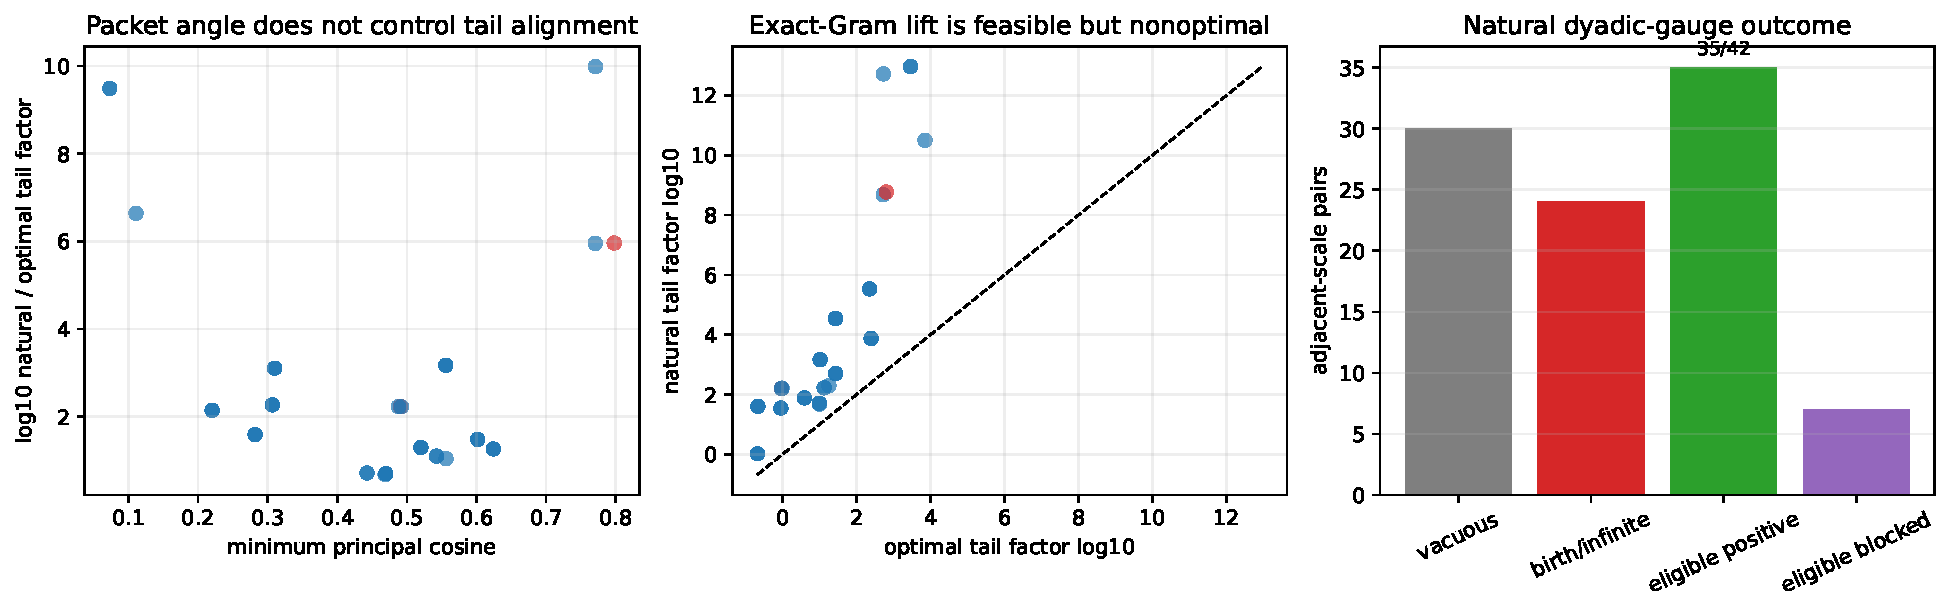
\includegraphics[width=\textwidth]{figures/dyadic_packet_transport_gauge.pdf}
\caption{Natural versus optimal tail transport.  Red points are the two
pairs positive under the minimax gauge but blocked by the natural gauge.}
\label{fig:audit}
\end{figure}

The positivity count is much better than the factor ratios alone suggest.
The 30 zero-to-zero pairs remain vacuously positive, and all 24 rank-birth
pairs remain infinite, as they must.  Of the 42 transport-eligible pairs, the
post-hoc optimum is positive on 37 and the natural gauge on 35.  Therefore
the total count falls only from 67 to 65.

The two lost pairs are both left-channel final-phase cases.  On
$0.08\to0.04$ at threshold $10^{-4}$, the minimum principal cosine is still
$0.798$, but the natural factor is $5.89\times10^8$ versus optimal
$643$, producing $\gamma_{\rm nat}\approx296$.  On
$0.04\to0.02$ at threshold $10^{-8}$, the natural factor is $160.65$ versus
optimal $0.954$, producing $\gamma_{\rm nat}\approx3.95$.  The first case
is especially decisive: a visually coherent packet frame can be violently
misaligned with the normalized tail.

\section{Route consequence and boundary}
RH-133 supplies a genuine model-derived cross-scale gauge.  It uses the
existing dyadic grid identification, the source-seeded packet recursion, and
the four-direction frame; no tail eigenframe is consulted in its definition.
It preserves nearly all finite positive transfers, so the natural-gauge route
is not numerically dead.  At the same time, the $10^{9.99}$ worst loss and
Proposition~\ref{prop:noangle} rule out any proof based only on principal
angles.

The next paper should derive the tail discrepancy itself from the finite
memory recursion.  The desired identity is an affine decomposition of the
target normalized tail into a dyadically transported old component plus a
newly born memory slice and controlled frame-change terms.  Those terms must
feed explicit candidates for $\rho_n$ and $q_n$.

We have not proved a uniform principal-angle law, a uniform natural tail
factor, an all-level affine recurrence, a normalized-base liminf, uniform
Stage A, a Hilbert--Polya operator, zeta-zero identification, or the Riemann
Hypothesis.

\bibliographystyle{plainnat}
\bibliography{references}
\end{document}
